\chapter{Method}
This chapter details the methods used in this project. First, the significance of the research is outlined against the context of the literature review. Next, the datasets used for training and validation of models are described and compared. Then, the ...

\section{Significance of this research}
Most of the previous work on collaborative filtering (CF) tackled the problem of predicting user preferences using their interaction history. The most successful methods all involve the use of latent factor models which are capable of learning otherwise hidden properties in the users and items in CF datasets. Recently this type of approach has been adapted from matrix factorisation models to neural architectures which capture latent factors in embedding layers, while allowing for non-linearity in successive hidden layers. 

CF models, by definition, do not make use of meta data for predicting user preferences -- this is the domain of content-based models. However, meta data such as item genres are still useful to users for assessing recommendations provided to them. Users cannot be expected to trust recommendations provided to them, without having some sort of description of the recommended item. While CF has shown its ability to provide recommendations to users without using content attributes, descriptive features are still useful for users to make informed decisions on \textit{which} recommendations to choose.

The following research questions motivated this minor dissertation: RQ1 -- can transfer learning be used to re-purpose a rating prediction model to predict item genres? RQ2 -- How does the choice of hyperparameters in the rating prediction model affect the performance of the genre prediction model?

\section{Datasets used}
There were five different datasets used in this research project, all of which contain explicit ratings made by users across various item sets. Three datasets contain movie ratings, while the other two contain ratings of books and jokes respectively.

The MovieLens datasets are used frequently in CF research efforts. GroupLens research at the university of Minnesota is responsible for maintaining these data in four stable sets of different sizes: 100K, 1M, 10M and 20M. For the purposes of this research, the 20M was not necessary and so only the first three were used. Each set is named after the number of ratings it contains. The first two datasets use a 5 star, integer-only rating scale, while the 10M and 20M datasets each contain ratings from 0.5 - 5 stars, including half star ratings \parencite{harper2016movielens}.

The Jester dataset contains over 4.1 million ratings of 100 jokes from over 70 000 users. Ratings fall on a continuous scale between -10 and +10. The low number of items and the continuous ratings scale make this dataset notably different to the others used in this project \parencite{cf_1.2_eigentaste}.

The goodbooks-10k dataset takes its name after the fact that it contains 10 000 books, rated a total of just under 6 million times by over 50 000 users \parencite{goodbooks2017}.

\subsection{Number of users, items and ratings}
Each dataset has a different profile in terms of the ratios between numbers of users, items and ratings. The density is calculated as the number of ratings provided as a proportion of the total number of possible user-item interactions. ML 100K -- the dataset with the fewest ratings -- has 943 unique users and 1 682 unique movie titles. This would allow a total of 1 586 126 possible user-movie ratings. Since there are only 100 000 ratings in this dataset, its density is thus $\dfrac{100000}{1.586126} = 6.30\%$. Table \ref{tab:data-summary} provides a summary of these datasets. 

\begin{table}[H]
\caption[Data summary]{Summary of the datasets used in this project}
\label{tab:data-summary}
\centering
\begin{tabular}{c | c | c | c | c | c}
\toprule
\textbf{Name} & \textbf{Rating Scale} & \textbf{Users} & \textbf{Items} & \textbf{Ratings} & \textbf{Density} \\
\midrule
ML 100K & 1--5, stars & 943 & 1 682 & 100 000 & 6.30\% \\
ML 1M & 1--5, stars & 6 040 & 3 706 & 1 000 209 & 4.47\% \\
ML 10M & 0.5--5, half-stars & 69 878 & 10 681 & 10 000 054 & 1.34\% \\
Jester & -10.0--10.0, decimal & 73 418 & 100 & 4 136 210 & 56.34\% \\
Goodbooks-10k & 1--5, stars & 53 424 & 10 000 & 5 976 479 & 1.12\% \\
\bottomrule
\end{tabular}
\end{table}

The Jester dataset has the highest density by a significant margin (56.34\%). ML 100K, 1M and the goodbooks-10k sets all use an integer rating scale between 1 and 5 stars. The ML 10M set also uses a 5 star scale, but allows half star ratings, whereas the Jester dataset uses a continuous ratings scale between -10 and +10.

In terms of size, ML 100K is ten times smaller than the second smallest ML 1M set, while the largest set is ML 10M with 10 million ratings. The Jester data set contains the most users, while ML 10M contains the most items, albeit only by a slight margin over goodbooks-10k.

\subsection{Distribution of ratings}
Table \ref{tab:ratings-distribution} provides a summary of the distribution of ratings across users and items in each of the datasets.

\begin{table}[H]
\caption[Ratings distribution]{Summary of the distribution of ratings in each dataset}
\label{tab:ratings-distribution}
\centering
\begin{tabular}{c | c | c | c | c | c | c}
\toprule
\textbf{Name} & \textbf{Min User} & \textbf{Max User} & \textbf{Avg User} & \textbf{Min Item} & \textbf{Max Item} & \textbf{Avg Item} \\
\midrule
ML 100K & 20 & 737 & 106 & 1 & 583 & 60 \\
ML 1M & 20 & 2 314 & 166 & 1 & 3 428 & 270 \\
ML 10M & 20 & 7 359 & 143 & 1 & 34 864 & 937 \\
Jester & 15 & 100 & 56 & 18 505 & 73 410 & 41 362 \\
Goodbooks-10k & 19 & 200 & 112 & 8 & 22 806 & 598 \\
\bottomrule
\end{tabular}
\end{table}

All three MovieLens datasets have a minimum of 20 ratings per user, while some of the movies have only 1 rating.

The Jester dataset has the fewest average ratings per user; however, each item is rated over 41-thousand times on average, with even the least frequently rated item having over 18-thousand ratings.

\textbf{put some plots here}...

\begin{figure}[H]
\centering
\begin{minipage}[b]{0.7\textwidth}
   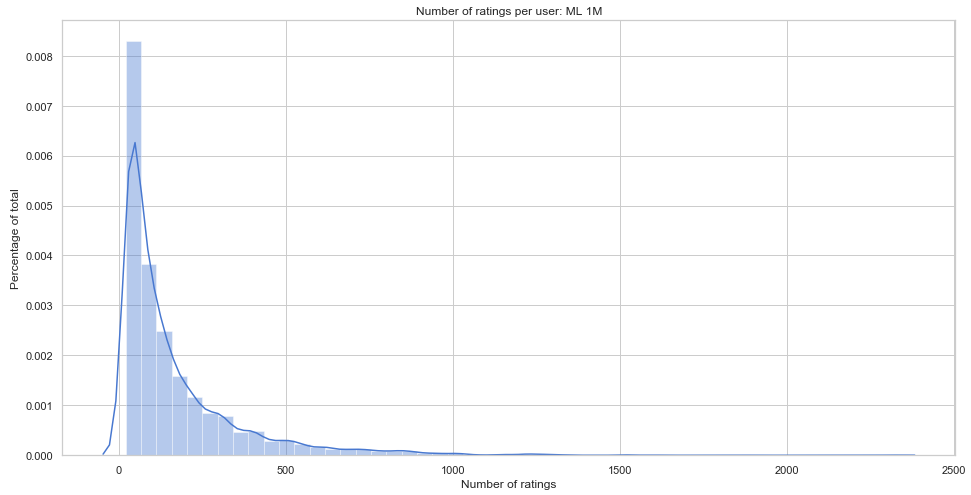
\includegraphics[width=1\linewidth]{Figures/ML1M-user-ratings.png}
   \caption{ML 1M distribution of user ratings}
   \label{fig:ML1m-users} 
\end{minipage}
\begin{minipage}[b]{0.7\textwidth}
   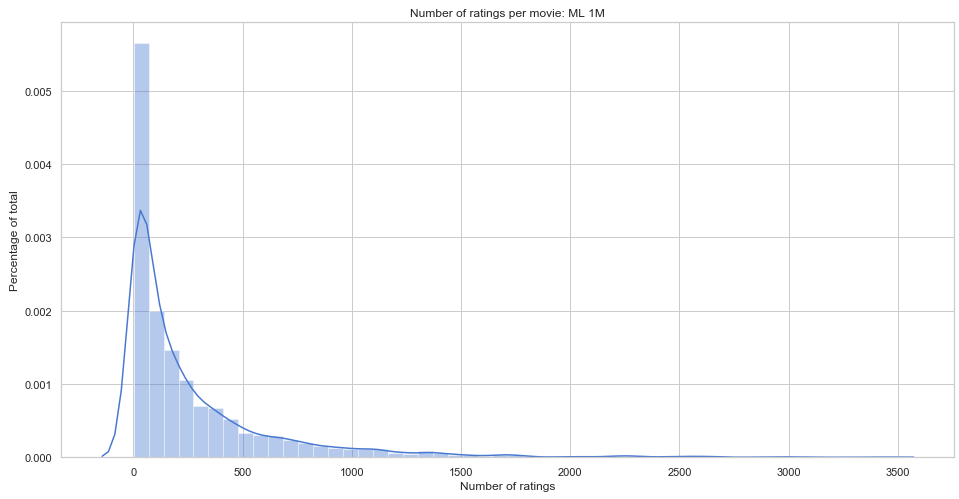
\includegraphics[width=1\linewidth]{Figures/ML1M-movie-ratings.png}
   \caption{ML 1M distribution of user ratings}
   \label{fig:ML1m-movies}
\end{minipage}
\end{figure}

\section{Predicting genres from ratings}
The process of predicting genres from explicit user-item interactions requires two steps. First, train a latent factor CF model to predict ratings. Then capture the item latent factors learnt by the model and use them to train a second model capable of mapping item latent factors to genres.

\section{Ratings prediction}

\subsection{Embedding layers}

\subsection{Model architecture}
\begin{figure}[H]
\centering
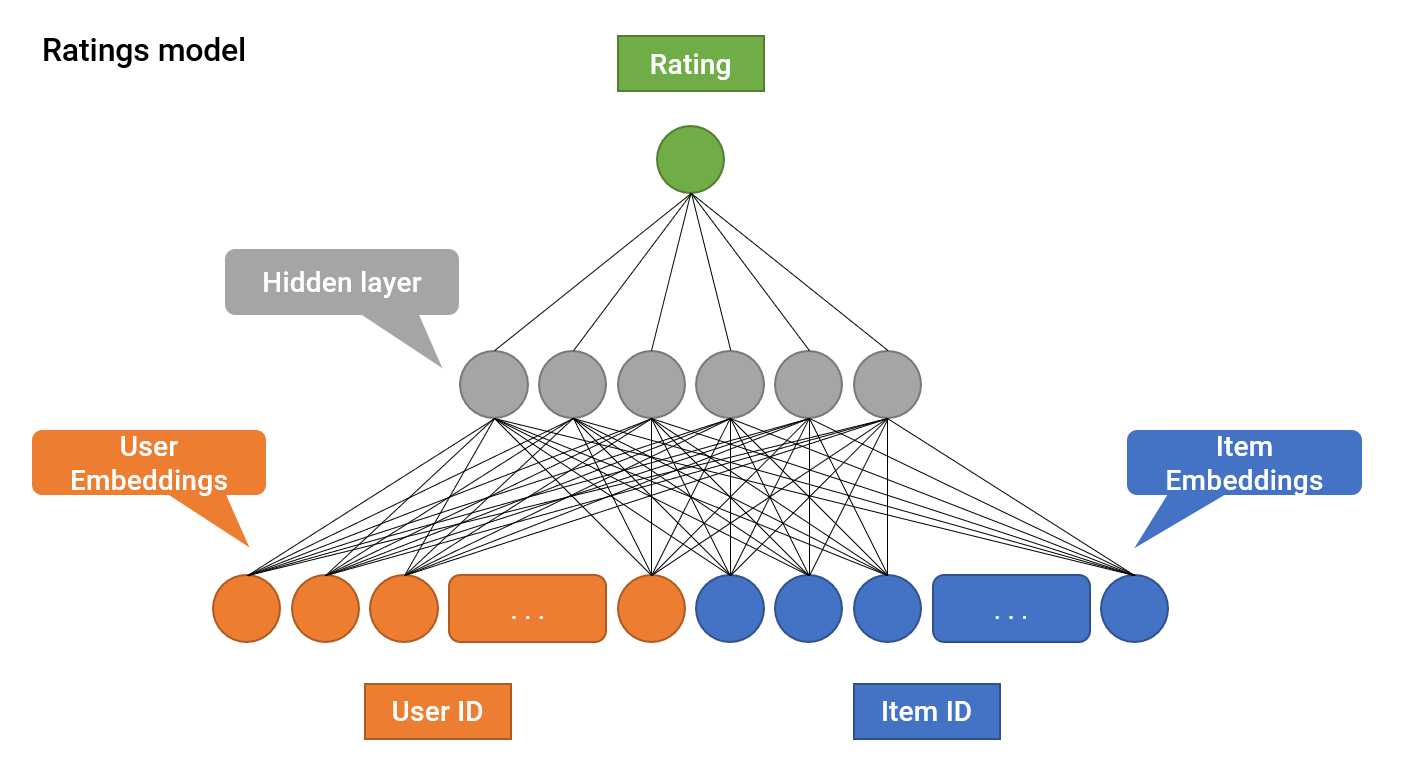
\includegraphics[width=0.9\textwidth]{Figures/3_ratings-model.png}
\decoRule
\caption[Ratings prediction model]{Rating prediction model uses embeddings to capture latent factors of items and users}
\label{fig:3_rating-prediction-architecture}
\end{figure}

\subsection{Hyper parameters}

\section{Genre prediction}

\subsection{Model architecture}
\begin{figure}[H]
\centering
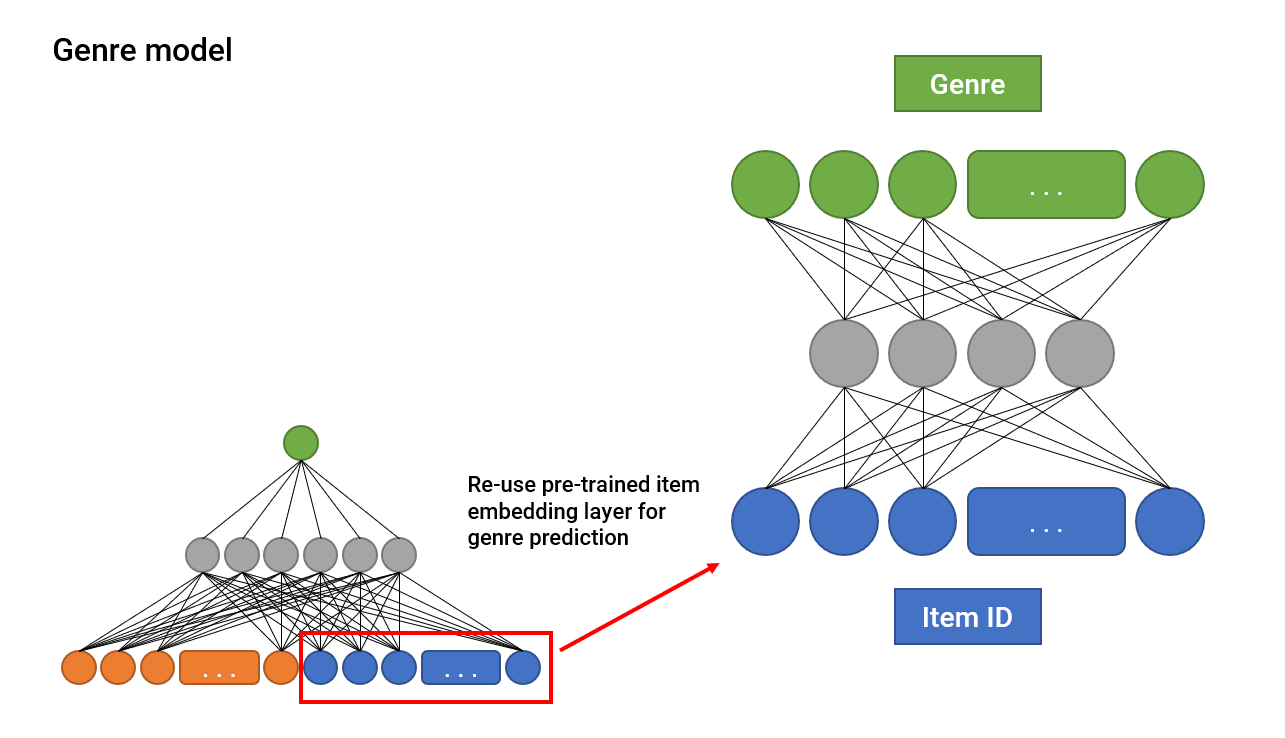
\includegraphics[width=0.9\textwidth]{Figures/3_genre-model.png}
\decoRule
\caption[Genre prediction model]{Genre prediction model re-uses the item embedding layer from the base ratings prediction model}
\label{fig:3_genre-prediction-architecture}
\end{figure}

\subsection{Hyper parameters}